% Szkielet dla pracy dyplomowej
%wybrać jeden z poniższych typów dokumentów:
\documentclass[english, polish, bachelor, a4paper,oneside]{ppciethesis} %praca inżynierska w j. polskim
%\documentclass[english, polish, a4paper,oneside]{ppciethesis} %praca inżynierska w j. polskim
%\documentclass[polish, english, bachelor, a4paper,oneside]{ppciethesis} %bachelors thesis in english
%\documentclass[polish, english, a4paper,oneside]{ppciethesis} %masters thesis in english

\usepackage{polski}%comment this if you are writing in english
\usepackage[utf8]{inputenc}

%\usepackage[OT4]{fontenc}

\usepackage{hyperref}
\usepackage{subfig}
\usepackage{float}
\usepackage{amsfonts}
\usepackage{pdfpages}
\usepackage{listings}

\linespread{1}

\author{Tomasz Kostur \and Grzegorz Zachar} % Your name comes here
\title{Format pracy dyplomowej (projekt~zespołowy)} % Note how we protect the final title phrase from breaking
\ppsupervisor{dr~hab.~inż.~(Marek Kraft)~profesor~nadzwyczajny} % Your supervisor comes here.
\ppyear{2015}  % Year of final submission %(not graduation!)


\begin{document}

\bibliographystyle{plplain}

% Front matter starts here
\frontmatter\pagestyle{empty}%
\maketitle
\cleardoublepage%
\Large

\thispagestyle{empty}\vspace*{\fill}
\cleardoublepage

% Blank info page for "karta dyplomowa"
\thispagestyle{empty}\vspace*{\fill}%
\begin{center}Tutaj znajdzie się karta pracy dyplomowej;\\oryginał wstawiamy do wersji dla archiwum PP, w pozostałych kopiach wstawiamy ksero.\end{center}%
\vfill
\cleardoublepage

\noindent
Podziękowania:\\ \\
\noindent
W tym miejscu można wstawić podziękowania.\\
Imię i Nazwisko autora 1
\\ \\
\noindent
Lub nie wstawiać żadnych.\\
Imię i Nazwisko autora 2
\\
\cleardoublepage
\thispagestyle{empty}\vspace*{\fill}
\cleardoublepage

% Table of contents.
\pagenumbering{Roman}\pagestyle{ppfcmthesis}%
\tableofcontents* \cleardoublepage%

\begin{abstract}
Obiektem badań pracy jest układ scalony Xillinx Zynq 7000.
Jest on przedstawicielem nowego typu układów scalonych łączących w sobie
sekwęcyjny mikroprocesor z programowalnym układem fpga.

Praca przedstawia sposób projektowania oprogramowania tego typu układów w połączeniu
z systemem operacyjnym linux.
Aplikacją realizowaną na układzie jest prosty algorytm stereowizyjny.
Praca zawiera porówania różnego rodzaju implementacji algorytmu, realizowanego
przy biblioteki OpenCV własnej logiki programowalnej oraz dostarczonego przez
xillinx DMA implementowanego w fpga. Praca opisuje wady i zalety używania
systemu linux, licznie napotkane problemy programistyczne lub błędy oprogramowania.
Praca wskazóje na wiele możliwości optymalizacji aplikacji oraz przedstawia benchmark
uzyskanych wyników
\end{abstract}

{
\selectlanguage{english}
\begin{abstract}
In this thesis example format of Institute of Control and Information Engineering thesis is presented.
\end{abstract}
}
\cleardoublepage

% Main content of your thesis starts here.
\mainmatter%
\chapter{Wstęp}
\label{sec:wstep}
\textit{Autor: Mateusz Kowalski}

%===============================================================================
\section{Zawartość wstępu}
\label{sec:wstep:co}

\subsection{Opis zagadnienia poruszonego w pracy}
\sloppy
Pierwszy rozdział pracy powinien zawierać opis zagadnienia poruszonego w pracy.

\subsection{Rys historyczny i aktualne zastosowania}
\label{sec:wstep:rys}

Można również opisać historię badañ danego tematu, oraz jego aktualnych zastosowañ.

\subsection{Autorstwo pracy}
\textit{Autor: Rafał Kabaciñski}\\ \\
W przypadku pracy zespołowej pod tytułem każdego rozdziału powinno znaleźć się imię i nazwisko autora danego rozdziału. Autorem rozdziału może być tylko jedna osoba, ale podrozdziały mogą mieć innego autora niż cały rozdział. 

%===============================================================================
\section{Cel pracy}
\label{sec:wstep:cel}

	Wstęp powienien zawierać również rozdział opisujący cele projektu opisywanego w pracy jak na przykład:
	
\begin{itemize}
	\item zapoznanie się z informacjami na temat istniejących rozwiązañ,
	\item stworzenie funkcjonalnego urządzenia,
	\item sprawdzenie wybranych rozwiązañ konstrukcyjnych.
\end{itemize}

\section{Zawartość pracy}
\label{sec:wstep:zawartosc}
	
	Ostatecznie wstęp musi zawierać przewodnik opisujący co znajduje się w dalszych rozdziałach pracy. Na przykład:
	Ogólny zarys stanu wiedzy na temat przygotowania i składu prac dyplomowych przedstawiono w rozdziale drugim. W rozdziale trzecim wprowadzono podstawowe informacje na temat korzystania z tego formatu pracy. Rozdział czwarty stanowi podsumowanie pracy.

\chapter{Stan wiedzy}
\label{sec:stanwiedzy}

Oprócz rozdziału opisującego rys historyczny (\ref{sec:wstep:rys}) konieczne jest również opisanie stanu wiedzy na temat danego zagadnienia. Powinno ono siê znaleźć w rozdziale drugim.

\section{Informacje dotyczące redakcji prac dyplomowych}
\label{sec:stanwiedzy:redakcja}

Informacje dotyczące zasad redakcji prac dyplomowych można znaleźć na stronie \url{www.cie.put.poznan.pl}.

\chapter{Treść pracy}
\label{sec:tresc}

\section{Użwanie pakietu \LaTeX}
\label{sec:tresc:latex}

	Informacje o tym jak używać pakietu \LaTeX można znaleźć w \cite{wiki:latex} i \cite{latex1}.\\

\section{Podział pracy na osobne pliki}
\label{sec:tresc:podzial}

Aby ułatwić pracę nad dokumentem, zwłaszcza w przypadku większej liczby zespołów warto go podzielić na większą ilość plików, na przykład według rozdziałów. W takim przypadku poszczególne rozdziały będą napisane w osobnych plikach tex, wstawianych do dokumentu głównego poleceniem $\backslash input$, na przykład:

%przykład wstawiania kodu:
\begin{lstlisting}
%\chapter{Wstęp}
\label{sec:wstep}
\textit{Autor: Mateusz Kowalski}

%===============================================================================
\section{Zawartość wstępu}
\label{sec:wstep:co}

\subsection{Opis zagadnienia poruszonego w pracy}
\sloppy
Pierwszy rozdział pracy powinien zawierać opis zagadnienia poruszonego w pracy.

\subsection{Rys historyczny i aktualne zastosowania}
\label{sec:wstep:rys}

Można również opisać historię badañ danego tematu, oraz jego aktualnych zastosowañ.

\subsection{Autorstwo pracy}
\textit{Autor: Rafał Kabaciñski}\\ \\
W przypadku pracy zespołowej pod tytułem każdego rozdziału powinno znaleźć się imię i nazwisko autora danego rozdziału. Autorem rozdziału może być tylko jedna osoba, ale podrozdziały mogą mieć innego autora niż cały rozdział. 

%===============================================================================
\section{Cel pracy}
\label{sec:wstep:cel}

	Wstęp powienien zawierać również rozdział opisujący cele projektu opisywanego w pracy jak na przykład:
	
\begin{itemize}
	\item zapoznanie się z informacjami na temat istniejących rozwiązañ,
	\item stworzenie funkcjonalnego urządzenia,
	\item sprawdzenie wybranych rozwiązañ konstrukcyjnych.
\end{itemize}

\section{Zawartość pracy}
\label{sec:wstep:zawartosc}
	
	Ostatecznie wstęp musi zawierać przewodnik opisujący co znajduje się w dalszych rozdziałach pracy. Na przykład:
	Ogólny zarys stanu wiedzy na temat przygotowania i składu prac dyplomowych przedstawiono w rozdziale drugim. W rozdziale trzecim wprowadzono podstawowe informacje na temat korzystania z tego formatu pracy. Rozdział czwarty stanowi podsumowanie pracy.

%\chapter{Stan wiedzy}
\label{sec:stanwiedzy}

Oprócz rozdziału opisującego rys historyczny (\ref{sec:wstep:rys}) konieczne jest również opisanie stanu wiedzy na temat danego zagadnienia. Powinno ono siê znaleźć w rozdziale drugim.

\section{Informacje dotyczące redakcji prac dyplomowych}
\label{sec:stanwiedzy:redakcja}

Informacje dotyczące zasad redakcji prac dyplomowych można znaleźć na stronie \url{www.cie.put.poznan.pl}.

%\chapter{Treść pracy}
\label{sec:tresc}

\section{Użwanie pakietu \LaTeX}
\label{sec:tresc:latex}

	Informacje o tym jak używać pakietu \LaTeX można znaleźć w \cite{wiki:latex} i \cite{latex1}.\\

\section{Podział pracy na osobne pliki}
\label{sec:tresc:podzial}

Aby ułatwić pracę nad dokumentem, zwłaszcza w przypadku większej liczby zespołów warto go podzielić na większą ilość plików, na przykład według rozdziałów. W takim przypadku poszczególne rozdziały będą napisane w osobnych plikach tex, wstawianych do dokumentu głównego poleceniem $\backslash input$, na przykład:

%przykład wstawiania kodu:
\begin{lstlisting}
%\chapter{Wstęp}
\label{sec:wstep}
\textit{Autor: Mateusz Kowalski}

%===============================================================================
\section{Zawartość wstępu}
\label{sec:wstep:co}

\subsection{Opis zagadnienia poruszonego w pracy}
\sloppy
Pierwszy rozdział pracy powinien zawierać opis zagadnienia poruszonego w pracy.

\subsection{Rys historyczny i aktualne zastosowania}
\label{sec:wstep:rys}

Można również opisać historię badañ danego tematu, oraz jego aktualnych zastosowañ.

\subsection{Autorstwo pracy}
\textit{Autor: Rafał Kabaciñski}\\ \\
W przypadku pracy zespołowej pod tytułem każdego rozdziału powinno znaleźć się imię i nazwisko autora danego rozdziału. Autorem rozdziału może być tylko jedna osoba, ale podrozdziały mogą mieć innego autora niż cały rozdział. 

%===============================================================================
\section{Cel pracy}
\label{sec:wstep:cel}

	Wstęp powienien zawierać również rozdział opisujący cele projektu opisywanego w pracy jak na przykład:
	
\begin{itemize}
	\item zapoznanie się z informacjami na temat istniejących rozwiązañ,
	\item stworzenie funkcjonalnego urządzenia,
	\item sprawdzenie wybranych rozwiązañ konstrukcyjnych.
\end{itemize}

\section{Zawartość pracy}
\label{sec:wstep:zawartosc}
	
	Ostatecznie wstęp musi zawierać przewodnik opisujący co znajduje się w dalszych rozdziałach pracy. Na przykład:
	Ogólny zarys stanu wiedzy na temat przygotowania i składu prac dyplomowych przedstawiono w rozdziale drugim. W rozdziale trzecim wprowadzono podstawowe informacje na temat korzystania z tego formatu pracy. Rozdział czwarty stanowi podsumowanie pracy.

%\chapter{Stan wiedzy}
\label{sec:stanwiedzy}

Oprócz rozdziału opisującego rys historyczny (\ref{sec:wstep:rys}) konieczne jest również opisanie stanu wiedzy na temat danego zagadnienia. Powinno ono siê znaleźć w rozdziale drugim.

\section{Informacje dotyczące redakcji prac dyplomowych}
\label{sec:stanwiedzy:redakcja}

Informacje dotyczące zasad redakcji prac dyplomowych można znaleźć na stronie \url{www.cie.put.poznan.pl}.

%\chapter{Treść pracy}
\label{sec:tresc}

\section{Użwanie pakietu \LaTeX}
\label{sec:tresc:latex}

	Informacje o tym jak używać pakietu \LaTeX można znaleźć w \cite{wiki:latex} i \cite{latex1}.\\

\section{Podział pracy na osobne pliki}
\label{sec:tresc:podzial}

Aby ułatwić pracę nad dokumentem, zwłaszcza w przypadku większej liczby zespołów warto go podzielić na większą ilość plików, na przykład według rozdziałów. W takim przypadku poszczególne rozdziały będą napisane w osobnych plikach tex, wstawianych do dokumentu głównego poleceniem $\backslash input$, na przykład:

%przykład wstawiania kodu:
\begin{lstlisting}
%\input{01-Wstep.tex}
%\input{02-Stanwiedzy.tex}
%\input{03-Tresc.tex}
%\input{04-Wnioski.tex}
\end{lstlisting}

\section{Wzory matematyczne w \LaTeX}
\label{sec:tresc:wzory}

Przykładowy wzór: odwrotna transformata Fouriera:

\begin{itemize}
\item Ciągła:

\begin{equation}
 f(x) = \mathcal{F}^{-1}\{\hat{f}(\xi)\} = \int\limits_{-\infty}^{\infty}\hat{f}(\xi)e^{2\pi ix\xi}dx
 \label{eq:f2}
\end{equation}

\item Dyskretna:

\begin{equation}
 f(n) = \frac{1}{N}\sum\limits_{k = 0}^{N-1}F_{DFT}(k)e^{j \frac{2\pi}{N}nk}dx
 \label{eq:f4}
\end{equation}

\end{itemize}

Przykładowa macierz: elementarna macierz obrotu punktu wokół osi $x$ o kąt $\alpha$:

$$RotX(\alpha) = \left[ \begin{array}{c c c} 
1 & 0 & 0 \\
0 & cos(\alpha) & -sin(\alpha) \\ 
0 & sin(\alpha) & cos(\alpha)
\end{array} \right] $$

\section{Tabele}
\label{sec:tresc:tab}

Tabela \ref{tab1} zawiera przykładowe wyniki dwóch sprawdzianów.

\begin{table}[h]
	\begin{center}
	\caption{Przykladowa tabela}
	\label{tab1}
	\begin{tabular}{|c|c|c|c|}
		\hline
		Lp.& nr indeksu & \multicolumn{2}{|c|}{kolokwium}\\ \cline{3-4}
		   &            & I   & II \\ \hline
		1  & 32453      & 4,0  & 5,0\\
		2  & 42546      & 3,5  & 4,0\\
		3  & 32546      & 2,0  & 3,0\\ \hline
	\end{tabular}
	\end{center}
\end{table}

\section{Rysunki}
\label{sec:tresc:rys}

Rysunek \ref{fig:rys1} zawiera logo Politechniki Poznañskiej.\\

\begin{figure}[h]
	\begin{center}
		
\includegraphics[height = 3cm]{figures/template/logo-pp}
		\caption[Logo Politechniki Poznañskiej]{Logo Politechniki Poznañskiej; uwaga: w podpisach rysunków nie ma kropek na koñcu zdania; jeżeli zdañ jest więcej należy oddzielać je średnikami i zaczynać z małej litery}

		\label{fig:rys1}
	\end{center}
\end{figure}

\section{Dodawanie pakietów}
\label{sec:tresc:pakiety}

W przypadku użycia pakietu MiKTeX, aby zainstalować dodatkowe pakiety należy włączyć {\itshape Package Manager}, w katalogu {\itshape Maintenance (Admin)}. Następnie w pole {\itshape Name} wpisać nazwę brakującego pakietu i nacisnąć przycisk {\itshape Filter}. Nazwę wybranego pakietu należy kliknąć prawym przyciskiem myszy i nacisnąć {\itshape Install}, jak na rysunku \ref{fig:pakiety}.

\begin{figure}[h]
	\begin{center}
		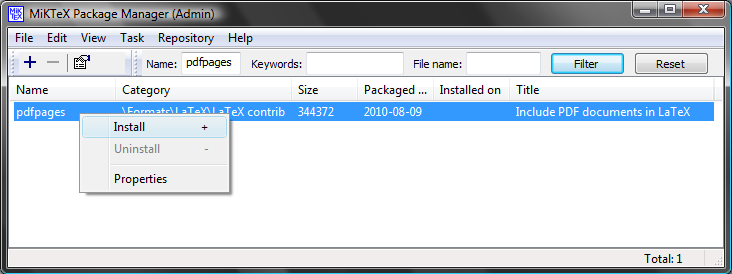
\includegraphics[width = 12cm]{figures/pakiety.png}
		\caption{Instalacja dodatkowych pakietów}
		\label{fig:pakiety}
	\end{center}
\end{figure}

\section{Pakiet Bib\TeX}
\label{sec:tresc:bibtex}

Pakiet Bib\TeX służy do zarządzania bibliografią. Pozycje bibliograficzne zapisywane są w plikach tekstowych z rozszerzeniem $.bib$, a następnie wywołanie poleceniem $\backslash cite$. Pliki bib muszą mieć odpowiednią strukturę, którą można poznać na stronie \url{http://pl.wikipedia.org/wiki/BibTeX}, lub \url{http://en.wikipedia.org/wiki/BibTeX}.\\
Bibliografię tworzy się wywołując w dokumencie polecenie $\backslash bibliography$. Po skompilowaniu dokumentu zawierającego odwołania do bibliografii, należy skompilować bibliografię za pomocą osobnego przycisku, a następnie znów skompilować dokument. Kompiluje się jednak zawsze tylko z widoku głównego dokumentu. Bib\TeX sam uporządkuje bibliografię według podanego stylu, zamieszczając tylko te pozycje które zostały zacytowane. Styl bibliografii ustawiany jest poleceniem $\backslash bibliographystyle$ przed wywołaniem pierwszego cytowania. W tym dokumencie użyto stylu plplain.

%
\chapter{Podsumowanie}
\label{sec:podsumowanie}

W podsumowaniu należy pokrótce opisać sposoby i efekty realizacji celów pracy przedstawionych w rozdziale \ref{sec:wstep:cel}. Oprócz tego powinny siê tu znaleść wnioski wynikające z wyników pracy, oraz dalsze kierunki rozwoju zagadnienia.

\end{lstlisting}

\section{Wzory matematyczne w \LaTeX}
\label{sec:tresc:wzory}

Przykładowy wzór: odwrotna transformata Fouriera:

\begin{itemize}
\item Ciągła:

\begin{equation}
 f(x) = \mathcal{F}^{-1}\{\hat{f}(\xi)\} = \int\limits_{-\infty}^{\infty}\hat{f}(\xi)e^{2\pi ix\xi}dx
 \label{eq:f2}
\end{equation}

\item Dyskretna:

\begin{equation}
 f(n) = \frac{1}{N}\sum\limits_{k = 0}^{N-1}F_{DFT}(k)e^{j \frac{2\pi}{N}nk}dx
 \label{eq:f4}
\end{equation}

\end{itemize}

Przykładowa macierz: elementarna macierz obrotu punktu wokół osi $x$ o kąt $\alpha$:

$$RotX(\alpha) = \left[ \begin{array}{c c c} 
1 & 0 & 0 \\
0 & cos(\alpha) & -sin(\alpha) \\ 
0 & sin(\alpha) & cos(\alpha)
\end{array} \right] $$

\section{Tabele}
\label{sec:tresc:tab}

Tabela \ref{tab1} zawiera przykładowe wyniki dwóch sprawdzianów.

\begin{table}[h]
	\begin{center}
	\caption{Przykladowa tabela}
	\label{tab1}
	\begin{tabular}{|c|c|c|c|}
		\hline
		Lp.& nr indeksu & \multicolumn{2}{|c|}{kolokwium}\\ \cline{3-4}
		   &            & I   & II \\ \hline
		1  & 32453      & 4,0  & 5,0\\
		2  & 42546      & 3,5  & 4,0\\
		3  & 32546      & 2,0  & 3,0\\ \hline
	\end{tabular}
	\end{center}
\end{table}

\section{Rysunki}
\label{sec:tresc:rys}

Rysunek \ref{fig:rys1} zawiera logo Politechniki Poznañskiej.\\

\begin{figure}[h]
	\begin{center}
		
\includegraphics[height = 3cm]{figures/template/logo-pp}
		\caption[Logo Politechniki Poznañskiej]{Logo Politechniki Poznañskiej; uwaga: w podpisach rysunków nie ma kropek na koñcu zdania; jeżeli zdañ jest więcej należy oddzielać je średnikami i zaczynać z małej litery}

		\label{fig:rys1}
	\end{center}
\end{figure}

\section{Dodawanie pakietów}
\label{sec:tresc:pakiety}

W przypadku użycia pakietu MiKTeX, aby zainstalować dodatkowe pakiety należy włączyć {\itshape Package Manager}, w katalogu {\itshape Maintenance (Admin)}. Następnie w pole {\itshape Name} wpisać nazwę brakującego pakietu i nacisnąć przycisk {\itshape Filter}. Nazwę wybranego pakietu należy kliknąć prawym przyciskiem myszy i nacisnąć {\itshape Install}, jak na rysunku \ref{fig:pakiety}.

\begin{figure}[h]
	\begin{center}
		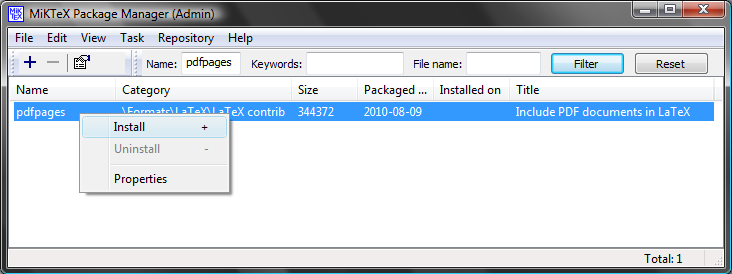
\includegraphics[width = 12cm]{figures/pakiety.png}
		\caption{Instalacja dodatkowych pakietów}
		\label{fig:pakiety}
	\end{center}
\end{figure}

\section{Pakiet Bib\TeX}
\label{sec:tresc:bibtex}

Pakiet Bib\TeX służy do zarządzania bibliografią. Pozycje bibliograficzne zapisywane są w plikach tekstowych z rozszerzeniem $.bib$, a następnie wywołanie poleceniem $\backslash cite$. Pliki bib muszą mieć odpowiednią strukturę, którą można poznać na stronie \url{http://pl.wikipedia.org/wiki/BibTeX}, lub \url{http://en.wikipedia.org/wiki/BibTeX}.\\
Bibliografię tworzy się wywołując w dokumencie polecenie $\backslash bibliography$. Po skompilowaniu dokumentu zawierającego odwołania do bibliografii, należy skompilować bibliografię za pomocą osobnego przycisku, a następnie znów skompilować dokument. Kompiluje się jednak zawsze tylko z widoku głównego dokumentu. Bib\TeX sam uporządkuje bibliografię według podanego stylu, zamieszczając tylko te pozycje które zostały zacytowane. Styl bibliografii ustawiany jest poleceniem $\backslash bibliographystyle$ przed wywołaniem pierwszego cytowania. W tym dokumencie użyto stylu plplain.

%
\chapter{Podsumowanie}
\label{sec:podsumowanie}

W podsumowaniu należy pokrótce opisać sposoby i efekty realizacji celów pracy przedstawionych w rozdziale \ref{sec:wstep:cel}. Oprócz tego powinny siê tu znaleść wnioski wynikające z wyników pracy, oraz dalsze kierunki rozwoju zagadnienia.

\end{lstlisting}

\section{Wzory matematyczne w \LaTeX}
\label{sec:tresc:wzory}

Przykładowy wzór: odwrotna transformata Fouriera:

\begin{itemize}
\item Ciągła:

\begin{equation}
 f(x) = \mathcal{F}^{-1}\{\hat{f}(\xi)\} = \int\limits_{-\infty}^{\infty}\hat{f}(\xi)e^{2\pi ix\xi}dx
 \label{eq:f2}
\end{equation}

\item Dyskretna:

\begin{equation}
 f(n) = \frac{1}{N}\sum\limits_{k = 0}^{N-1}F_{DFT}(k)e^{j \frac{2\pi}{N}nk}dx
 \label{eq:f4}
\end{equation}

\end{itemize}

Przykładowa macierz: elementarna macierz obrotu punktu wokół osi $x$ o kąt $\alpha$:

$$RotX(\alpha) = \left[ \begin{array}{c c c} 
1 & 0 & 0 \\
0 & cos(\alpha) & -sin(\alpha) \\ 
0 & sin(\alpha) & cos(\alpha)
\end{array} \right] $$

\section{Tabele}
\label{sec:tresc:tab}

Tabela \ref{tab1} zawiera przykładowe wyniki dwóch sprawdzianów.

\begin{table}[h]
	\begin{center}
	\caption{Przykladowa tabela}
	\label{tab1}
	\begin{tabular}{|c|c|c|c|}
		\hline
		Lp.& nr indeksu & \multicolumn{2}{|c|}{kolokwium}\\ \cline{3-4}
		   &            & I   & II \\ \hline
		1  & 32453      & 4,0  & 5,0\\
		2  & 42546      & 3,5  & 4,0\\
		3  & 32546      & 2,0  & 3,0\\ \hline
	\end{tabular}
	\end{center}
\end{table}

\section{Rysunki}
\label{sec:tresc:rys}

Rysunek \ref{fig:rys1} zawiera logo Politechniki Poznañskiej.\\

\begin{figure}[h]
	\begin{center}
		
\includegraphics[height = 3cm]{figures/template/logo-pp}
		\caption[Logo Politechniki Poznañskiej]{Logo Politechniki Poznañskiej; uwaga: w podpisach rysunków nie ma kropek na koñcu zdania; jeżeli zdañ jest więcej należy oddzielać je średnikami i zaczynać z małej litery}

		\label{fig:rys1}
	\end{center}
\end{figure}

\section{Dodawanie pakietów}
\label{sec:tresc:pakiety}

W przypadku użycia pakietu MiKTeX, aby zainstalować dodatkowe pakiety należy włączyć {\itshape Package Manager}, w katalogu {\itshape Maintenance (Admin)}. Następnie w pole {\itshape Name} wpisać nazwę brakującego pakietu i nacisnąć przycisk {\itshape Filter}. Nazwę wybranego pakietu należy kliknąć prawym przyciskiem myszy i nacisnąć {\itshape Install}, jak na rysunku \ref{fig:pakiety}.

\begin{figure}[h]
	\begin{center}
		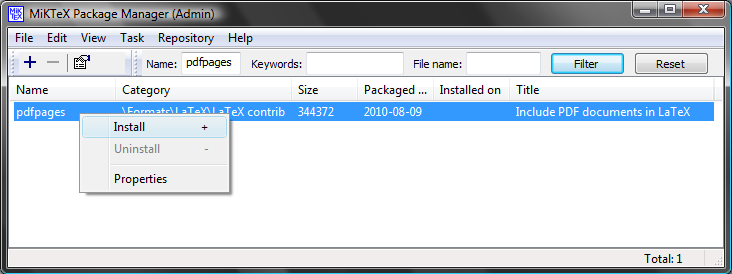
\includegraphics[width = 12cm]{figures/pakiety.png}
		\caption{Instalacja dodatkowych pakietów}
		\label{fig:pakiety}
	\end{center}
\end{figure}

\section{Pakiet Bib\TeX}
\label{sec:tresc:bibtex}

Pakiet Bib\TeX służy do zarządzania bibliografią. Pozycje bibliograficzne zapisywane są w plikach tekstowych z rozszerzeniem $.bib$, a następnie wywołanie poleceniem $\backslash cite$. Pliki bib muszą mieć odpowiednią strukturę, którą można poznać na stronie \url{http://pl.wikipedia.org/wiki/BibTeX}, lub \url{http://en.wikipedia.org/wiki/BibTeX}.\\
Bibliografię tworzy się wywołując w dokumencie polecenie $\backslash bibliography$. Po skompilowaniu dokumentu zawierającego odwołania do bibliografii, należy skompilować bibliografię za pomocą osobnego przycisku, a następnie znów skompilować dokument. Kompiluje się jednak zawsze tylko z widoku głównego dokumentu. Bib\TeX sam uporządkuje bibliografię według podanego stylu, zamieszczając tylko te pozycje które zostały zacytowane. Styl bibliografii ustawiany jest poleceniem $\backslash bibliographystyle$ przed wywołaniem pierwszego cytowania. W tym dokumencie użyto stylu plplain.


\chapter{Podsumowanie}
\label{sec:podsumowanie}

W podsumowaniu należy pokrótce opisać sposoby i efekty realizacji celów pracy przedstawionych w rozdziale \ref{sec:wstep:cel}. Oprócz tego powinny siê tu znaleść wnioski wynikające z wyników pracy, oraz dalsze kierunki rozwoju zagadnienia.


% All appendices and extra material, if you have any.
\cleardoublepage\appendix%
\chapter{Opis zawartości płyty DVD}

Zawartość płyty DVD lub CD dołączonej do pracy powinna zostać opisana w dodatku. Na płycie powinna znaleźć się cyfrową kopia pracy w formacie pdf.

\section{Przykładowy podrozdział dodatku}
\label{sec:dvd:przyk}
Dodatki mogą zawierać własne rozdziały, które nie ingerują w pozostałą strukturę dokumentu.

\chapter{Rysunki techniczne}

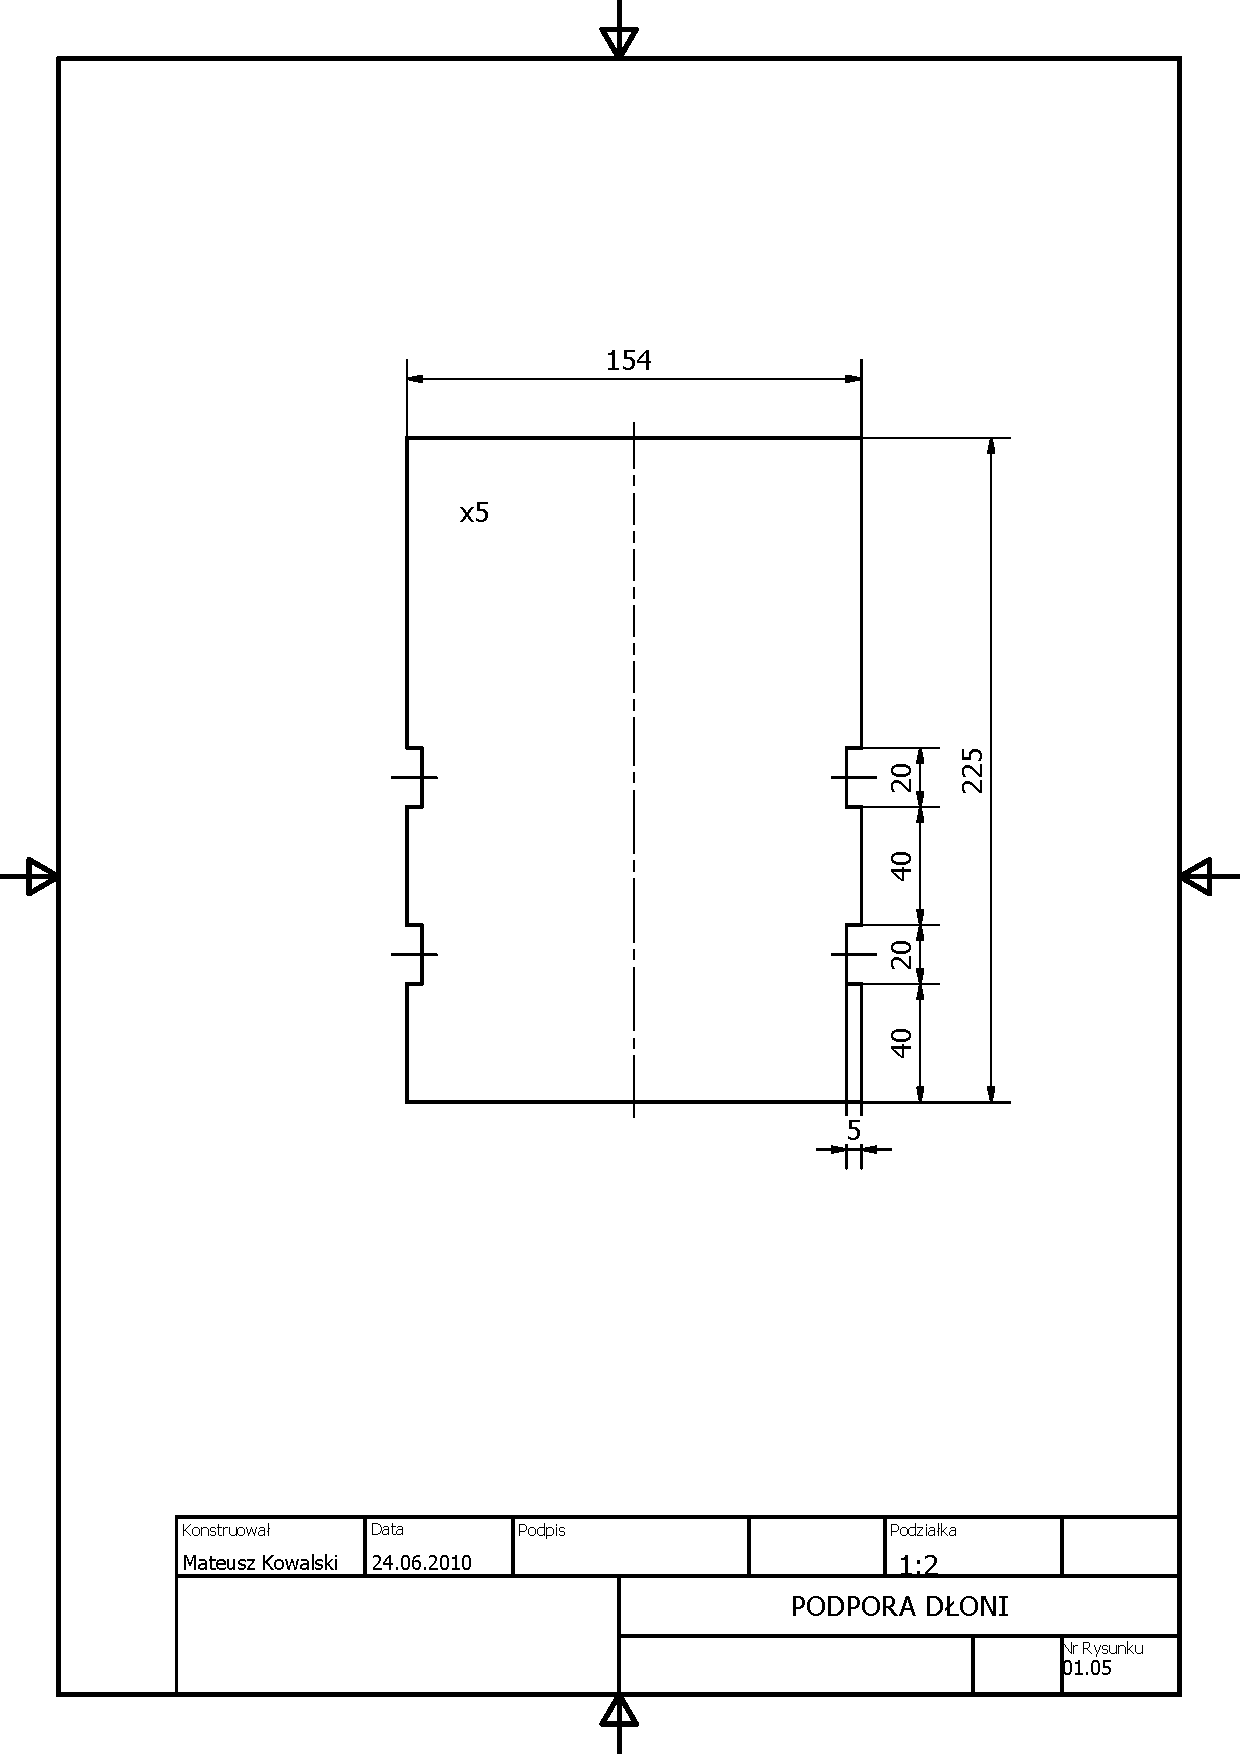
\includepdf{figures/podporadloni.pdf}


\cleardoublepage
\listoftables \cleardoublepage %lista tabel na osobnej stronie
\listoffigures \cleardoublepage %lista rysunków na osobnej stronie

% Bibliography (books, articles) starts here.
\bibliography{bibliografia}

% Colophon is a place where you should let others know about copyrights etc.
\ppcolophon

\end{document}
